\documentclass[thesis]{subfiles}

\begin{document}

\chapter{Podsumowanie}

W~tym rozdziale zostały przedstawione dalsze możliwe kierunki rozwoju zaimplementowanego rozwiązania oraz~wnioski wynikłe z~pracy przeprowadzonej nad~projektem.
%------------------------------------------------------------------------------

\section{Dalsze kierunki rozwoju}

\hyperref[sec:obraz-zmian-konfiguracji]{Obraz zmian konfiguracji systemu wzorcowego} tworzony przez \hyperref[sec:srv-app]{aplikację serwera}, zaimplementowaną w~ramach niniejszego projektu, może być dostarczony klientowi na~dwa sposoby --- ręcznie lub~automatycznie. Sposób ręczny polega na~tym, że~administrator przenosi taki obraz na~stację kliencką kopiując go ze~stacji serwera~np.~przez \href{https://en.wikipedia.org/wiki/Network_File_System}{NFS}, na~\hrefemph{http://sjp.pwn.pl/poradnia/haslo/Odmieniamy-pendrive;11159.html}{pendrivie} lub~w~dowolny inny sposób, po~czym uruchamia \hyperref[sec:cli-app]{aplikację kliencką}, która stosuje go~na~maszynie klienta. Sposób automatyczny działa w~ten sposób, że~aplikacja klienta jest uruchamiana przez \hreftt{https://en.wikipedia.org/wiki/Cron}{crona} co~jakiś czas i~zgłasza się ona do~innych klientów udostępniających taki obraz przez \sftp{}, a~następnie stosuje się do~niego.

Angażowanie klientów do~dystrybuowania wzorca oprogramowania, którego źródłem jest serwer, czyli system wzorcowy, może wydawać się nieadekwatne do~roli odgrywanej w~zaprojektowanym protokole przez klientów, dlatego w~alternatywnym modelu dystrybuowania jednakowego oprogramowania do~dużej ilości klientów można by było użyć rozwiązania opartego o~bezpołączeniowy model komunikacji między serwerem i~klientami, oparty o~\hrefemph{https://en.wikipedia.org/wiki/IP_multicast}{multicast}\footnote{Co~ciekawe, w~\href{https://en.wikipedia.org/wiki/IPv6}{IPv6} zrezygnowano z~\emph{broadcastu} na~rzecz \emph{multicastu}.}. Należy jednak pamiętać, że~warstwą transportową dla~metod multicastowych jest protokół~\href{https://en.wikipedia.org/wiki/User_Datagram_Protocol}{UDP}, który z~zasady działania jest zawodny, tzn.~nie gwarantuje, że~pakiety nie zostaną zduplikowane i~że~każdy wysłany pakiet dotrze do~celu, a~nawet jeśli dotrze, to~niekoniecznie w~takiej kolejności w~jakiej był wysłany~\cite{rfc1112}. Ponadto protokół~UDP nie uwzględnia m.in.~kontroli przepływu, tzn.~w~szczególności pakiety mogą przychodzić do~odbiorcy szybciej niż~ten może je~przetworzyć.

\begin{figure}
	\centering
	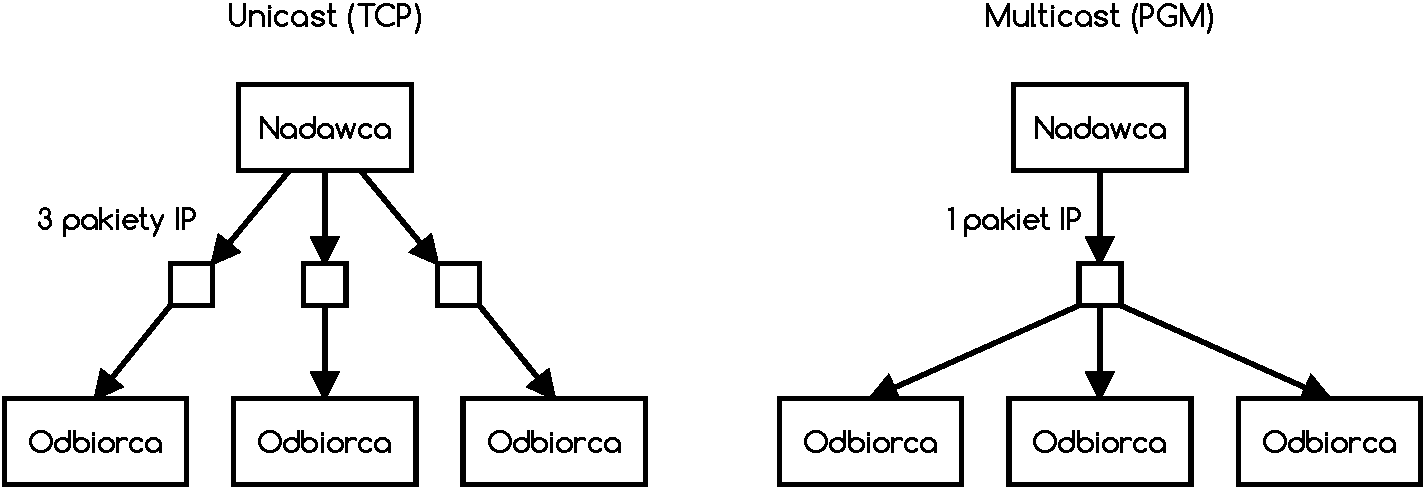
\includegraphics[width=0.8\textwidth]{img/unicast-vs-multicast}
	\caption[Zobrazowanie porównania unicastu i~multicastu]{Zobrazowanie porównania unicastu i~multicastu\\(na~podst.~\href{http://zeromq.wdfiles.com/local--files/whitepapers\%3Adesign-v05/pgm2.png}{rys.} opublikowanego na~stronie internetowej~\href{http://zeromq.org/}{ØMQ} na~warunkach licencji \glslink{copyleft}{copyleft} \href{https://creativecommons.org/licenses/by-sa/3.0/}{CC~BY-SA~3.0})}
	\label{fig:unicast-vs-multicast}
\end{figure}

Naturalną alternatywą dla~protokołu~UDP jest~TCP, jednak TCP, w~porównaniu do~UDP, jest złożonym protokołem połączeniowym warstwy transportowej, w~ramach którego przesyła się~wiele dodatkowych metadanych gwarantujących niezawodność połączenia, której nie zapewnia~UDP. Rozsyłanie przez serwer tej samej konfiguracji dużej liczbie klientów korzystając z~TCP wiąże się~z~nawiązywaniem połączenia z~każdym z~nich z~osobna, co~wydaje się być zbędne i~w~konsekwencji nieoptymalne~(por.~rys.~\ref{fig:unicast-vs-multicast}).

Kompromisem mógłby być taki podział zadań serwera w~protokole dystrybucji zadań, aby do~części z~nich wykorzystać protokół oparty na~TCP, a~do~pozostałej części protokół oparty na~UDP. Innym pomysłem mogłoby być wykorzystanie alternatywnego dla~TCP i~UDP protokołu warstwy transportowej. Jednym z~przykładów takiego protokołu jest~\href{https://en.wikipedia.org/wiki/QUIC}{QUIC}~(\emph{Quick UDP Internet Connections}) opracowany przez firmę Google i~stosowany domyślnie w~przeglądarce internetowej \href{https://www.google.pl/chrome/}{Chrome} do~\href{https://cs.chromium.org/chromium/src/net/tools/quic/quic_server.cc}{nawiązywania} połączeń ze~stronami internetowymi obsługiwanymi przez serwery Google. Celem projektowym QUIC było zminimalizowanie opóźnień w~protokole~TCP, upodabniając go~do UDP, jednocześnie zachowując zalety TCP i~dodając bezpieczeństwo połączenia oparte na~protokole~\gls{ssl/tls}~\cite{quic-wire-layout-spec,quic-crypto,quic-roskind}. W~czasie pisania tej~pracy QUIC nie jest jeszcze ustandaryzowany przez~\gls{ietf}, chociaż w~czerwcu~2016~roku powstał zespół, który pracuje nad~jego standaryzacją~\cite{quic-draft,quic-workinggroup}.

Innym przykładem alternatywnego protokołu warstwy transportowej jest~\href{https://en.wikipedia.org/wiki/Pragmatic_General_Multicast}{PGM}~(\emph{Pragmatic General Multicast}), który został zaprojektowany przez firmę \href{http://www.cisco.com/}{Cisco} z~myślą o~aplikacjach z~względnie prostymi wymaganiami dotyczącymi niezawodności, korzystających z~potencjału multicastu~\cite{pgm-rfc}. Założenia projektowe~PGM zostały przedstawione w~\href{https://tools.ietf.org/html/rfc3208}{RFC3208} i~są~bardzo bliskie potrzebom projektowanego protokołu, dlatego warstwą transportową zaprojektowanego w~ramach tej pracy rozwiązania mógłby być~PGM zaimplementowany np.~w~ramach projektu \href{https://code.google.com/archive/p/openpgm/}{OpenPGM} i~wykorzystany w~bibliotece~\href{http://zeromq.org/}{ØMQ}\footnote{Znanej też pod~nazwą~\hrefemph{http://zeromq.org/}{ZeroMQ}.}. Implementacja ta~\href{http://api.zeromq.org/2-1:zmq-pgm}{umożliwia} działanie~PGM w~dwóch trybach --- PGM oraz~ePGM~(\emph{Encapsulated PGM}). Pierwszy z~trybów implementuje wariant, w~którym datagramy PGM~są umieszczane bezpośrednio na~nagłówku~IP --- tak jak w~oryginalnym zamyśle~PGM, opisanym w~\href{https://tools.ietf.org/html/rfc3208}{RFC3208} --- a~drugi polega na~enkapsulacji datagramu~PGM w~datagramie~UDP, co~może być szczególnie użyteczne w~sieciach z~restrykcyjnymi \emph{firewallami}.

Kolejne dwa podrozdziały opisują szczegóły dotyczące protokołu~PGM i~jego możliwości w~kontekście alternatywnego wykorzystania w~komunikacji między serwerem i~klientem. Celem przygotowanego opisu jest przedstawienie, jak się wydaje\footnote{Przeczucia zweryfikowałyby testy.} --- lepszego, bo~szybszego i~lepiej skalowalnego --- modelu rozsyłania jednakowych zmian do~dużej liczby klientów.

%------------------------------------------------------------------------------

\subsection{Protokół PGM}
\label{subsec:pgm}

Problem braku standaryzacji protokołów niezawodnego multicastu został dostrzeżony przez organizację~\gls{ietf}, która jeszcze~w~latach~90. powołała zespoły \hrefemph{https://irtf.org/concluded/rmrg}{IRTF~Reliable Multicast Research Group} oraz~\hrefemph{https://ietf.org/wg/concluded/rmt}{Reliable Multicast Transport Working Group}, mające na~celu rozwiązywać problemy w~proponowanych protokołach niezawodnego multicastu~\cite{reliable-multicast-journal,reliable-multicast-transport}. Efektem prac tych zespołów są~dziesiątki dokumentów~\gls{rfc}, m.in.~\href{https://tools.ietf.org/html/rfc2357.html}{RFC2357} i~\href{https://tools.ietf.org/html/rfc2887}{RFC2887}, które określają wymagania jakie muszą spełniać protokoły niezawodnego multicastu~\cite{rfc2887,rfc2357}. Prace nad~niezawodnym multicastem prowadziły i~prowadzą również firmy, np.~Cisco --- autor~PGM.

Protokół \href{https://tools.ietf.org/html/rfc3208}{PGM}~(\emph{Pragmatic General Multicast}, a~pierwotnie \emph{Pretty Good Multicasting}) to~protokół do~rozgłaszania pakietów, korzystający z~multicastu, dzięki czemu wystarczy, że~w~czasie danej sesji rozgłoszeniowej, serwer wyśle tylko raz to, co~ma do~zakomunikowania swoim klientom~\cite{pgm-rfc}~(patrz~rys.~\ref{fig:unicast-vs-multicast}). Powielenie wiadomości do~wszystkich klientów, którzy zgłosili chęć otrzymywania multicastu odbywa się na~poziomie działania routera, do~którego klient jest podłączony bezpośrednio lub~pośrednio, tzn.~np.~za~pomocą przełączników sieciowych~(\emph{switchy}). Dołączenie i~opuszczenie grupy multicastowej przez klienta odbywa się w~sieciach IPv4 dzięki~protokołowi warstwy sieciowej \href{https://en.wikipedia.org/wiki/Internet_Group_Management_Protocol}{IGMP}~(\emph{Internet Group Management Protocol}), a~w~sieciach IPv6 dzięki protokołowi~\href{https://en.wikipedia.org/wiki/Multicast_Listener_Discovery}{MLD}~(\emph{Multicast Listener Discovery}), wbudowanemu w~protokół \href{https://en.wikipedia.org/wiki/Internet_Control_Message_Protocol_version_6}{ICMPv6}~(\emph{Internet Control Message Protocol version~6}). Protokół IGMP~istnieje w~trzech wersjach: IGMPv1, IGMPv2, IGMPv3 --- opisanych odpowiednio w~dokumentach:~\href{https://tools.ietf.org/html/rfc1112}{RFC1112}, \href{https://tools.ietf.org/html/rfc2236}{RFC2236} i~\href{https://tools.ietf.org/html/rfc3376}{RFC3376} (zaktualizowany przez~\href{https://tools.ietf.org/html/rfc4604}{RFC4604}). Protokół MLD~został opisany~w~\href{https://tools.ietf.org/html/rfc3810}{RFC3810} i~został zaktualizowany w~\href{https://tools.ietf.org/html/rfc4604}{RFC4604}.

Protokół~PGM różni się od~zwykłego multicastu opartego na~protokole~UDP m.in.~tym, że~pakiety zostają oznaczone sekwencyjnie liczbami całkowitymi, dzięki czemu klienci są~w~stanie stwierdzić czy~jakieś pakiety zostały ,,zgubione'' i~wymagają retransmisji. Jeśli klient wykryje, że~nie otrzymał wszystkich pakietów, ma~możliwość przez pewien, z~góry zdefiniowany czas\footnote{Formalnie okno czasowe (\emph{Transmit Window}), w~ramach którego klient może poprosić o~retransmisję pakietów, może być zdefiniowane za~pomocą czasu, liczby bajtów lub~liczby pakietów.}, wysłać prośbę o~retransmisję zadanych pakietów. W~przeciwieństwie do~protokołu UDP, PGM~gwarantuje, że~klient albo odbierze wszystkie pakiety i~ich ewentualne retransmisje, albo wykryje nieodwracalną utratę pakietów.

W~PGM każde źródło multicastu ma~przydzielony unikalny identyfikator TSI~(\emph{Transport Session Identifier}) będący wynikiem konkatenacji identyfikatora~GSI\footnote{\href{https://tools.ietf.org/html/rfc3208\#page-33}{RFC3208~zaleca}, aby~za~GSI przyjąć wartość funkcji mieszającej~\href{https://en.wikipedia.org/wiki/MD5}{MD5} dla~48~najmłodszych (najmniej znaczących) bitów \href{https://tools.ietf.org/html/rfc2535\#section-4}{sygnatury~DNS} serwera.}~(\emph{Global Source~ID}) oraz~portu używanego przez serwer. Podczas normalnego działania protokołu PGM, serwer wysyła multicastem dane do~klientów w~pakietach \texttt{ODATA}\footnote{Nazwa pakietu \texttt{ODATA} i~inne nazwy pakietów PGM przywołane w~tym rozdziale pochodzą z~\href{https://tools.ietf.org/html/rfc3208}{RFC3208}, definiującego protokół~PGM.} (\emph{Original Data}), a~klienci, jeśli wykryją brakujące pakiety, wysyłają unicastem do~ostatniego routera na~drodze od~serwera do~klienta pakiet \texttt{NAK}~(\emph{Negative Acknowledgment}) tak długo, jak długo nie otrzymają w~odpowiedzi pakietu \texttt{NCF}~(\emph{NAK Confirmation}). Serwer numeruje kolejnymi liczbami całkowitymi (cyklicznie) z~zakresu~$[0,~2^{32}-1]$ każdy kolejny pakiet \texttt{ODATA} z~danymi przekazanymi przez warstwę aplikacji. Router który otrzyma pakiet \texttt{NAK} przekazuje go do~routera poziom wyżej w~hierarchii sieciowej lub, jeśli router jest podłączony bezpośrednio do~serwera, przekazuje go~serwerowi. Na~każdym poziomie przekazywania \texttt{NAK} w~górę drzewa, którego korzeniem jest serwer, zostaje rozesłany multicastem pakiet \texttt{NCF} tylko na~tym interfejsie, na~którym przyszedł pakiet~\texttt{NAK}. Pakiety \texttt{NAK} pokonują dokładnie tą~samą drogę co~dane \texttt{ODATA}, tylko od~końca, co~jest ważne dla~przesyłanych pakietów naprawczych \texttt{RDATA}~(\emph{Repair Data}), ponieważ routery otrzymując~\texttt{NAK} zapamiętują m.in.~to, że~otrzymały taki pakiet i~numer interfejsu na~którym go~otrzymały, ustanawiając stan naprawczy~(\emph{Repair State}). Jeśli pakiet naprawczy \texttt{RDATA} zostałby wysłany do~routera, który nie ma ustawionego stanu naprawczego, to~zostałby zignorowany. Pomiędzy pakietami \texttt{ODATA} są~co~jakiś czas przesyłane pakiety \texttt{SPM}~(\emph{Source Path Messages}), dzięki którym pakiety \texttt{NAK} wracają dokładnie tą~ścieżką od~klienta do~serwera, którą zostałby wysłany pakiet \texttt{ODATA}. W~szczególności, dzięki~\texttt{SPM} klient wie który router obsługujący~PGM jest ostatni na~drodze od~źródła do~niego samego i~do~tego właśnie routera kieruje unicastem pakiety~\texttt{NAK}. Klient nie może prosić serwer o~retransmisję żadnego pakietu dopóki nie odbierze co~najmniej jednego pakietu~\texttt{SPM}. ,,Zgubione'' pakiety są~retransmitowane w~odpowiedzi na~pakiety \texttt{NAK} pakietami \texttt{RDATA} przez serwer lub~tzw.~DLR~(\emph{Designated Local Repairer}), którym może być któryś z~routerów obsługujących~protokół PGM.

Rysunek~\ref{fig:NAKflow} przedstawia diagram reprezentujący maszynę stanu dla~algorytmu wysyłania przez klienta pakietu~\texttt{NAK}. Odbiór pakietu \texttt{RDATA} lub~\texttt{ODATA} w~dowolnym stanie powoduje natychmiastowe przejście do~stanu terminalnego (niezaznaczonego na~rys.~\ref{fig:NAKflow}), zakończonego sukcesem. Stan \texttt{BACK\_OFF-STATE} trwa przez pewien, losowany z~pewnego przedziału, czas \texttt{NAK\_RB\_IVL} i~służy zmniejszeniu obciążenia sieci przez wykrycie ewentualnych odpowiedzi~\texttt{NCF}\footnote{Wysłanych w~reakcji na~pakiety~\texttt{NAK} innych klientów.} dotyczących pakietów, które klient chce otrzymać. Stan \texttt{WAIT\_NCF\_STATE} reprezentuje czas \texttt{NAK\_RPT\_IVL} przez który klient oczekuje na~odpowiedź~\texttt{NCF} --- jeśli jej nie otrzymana, to~wysyłany jest kolejny pakiet~\texttt{NAK}. Stan \texttt{WAIT\_DATA\_STATE} reprezentuje czas przez który klient czeka na~dane~\texttt{RDATA} --- jeśli ich nie otrzyma, to~cały proces zaczyna się od~nowa.

\begin{figure}
	\centering
	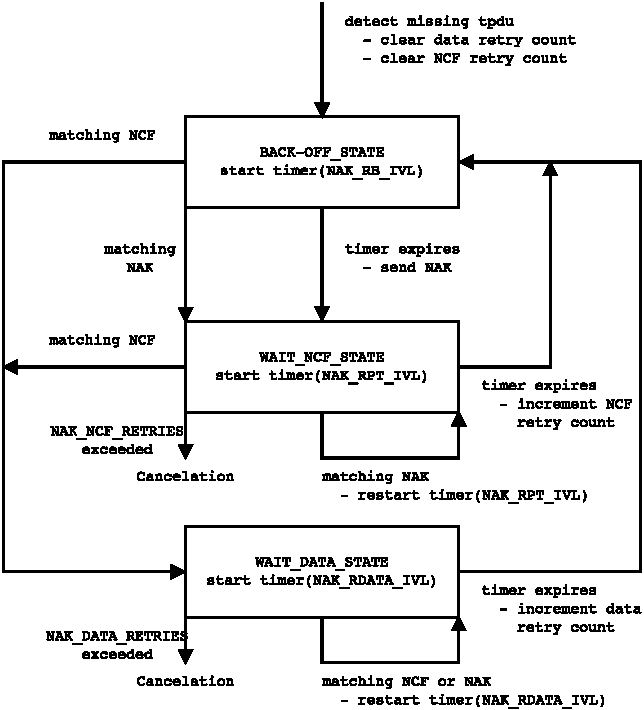
\includegraphics[width=0.62\textwidth]{img/PGF_protocol_NAK_flow_diagram}
	\caption[Diagram stanów dla~procesu generowania pakietów~\texttt{NAK} w~protokole~PGM]{Diagram stanów dla~procesu generowania pakietów~\texttt{NAK} w~protokole~PGM~(źródło:~\href{https://tools.ietf.org/html/rfc3208\#page-25}{RFC3208})~\cite{pgm-rfc}}
	\label{fig:NAKflow}
\end{figure}

Schemat pamięci pakietów \texttt{ODATA} i~\texttt{RDATA} został przedstawiony na~rysunku~\ref{fig:odata-packet}. Pierwsze 32~bajty to~pola wspólne dla~wszystkich typów pakietów w~protokole~PGM, czyli nagłówek pakietu. W~skład nagłówka wchodzą:\mynobreakpar

\begin{itemize}
	\item \texttt{Source~Port} (2~bajty) --- port źródłowy serwera~(tak jak w~nagłówku~UDP).
	\item \texttt{Destination~Port} (2~bajty) --- port docelowy klienta~(tak jak w~nagłówku~UDP).
	\item \texttt{Type} (1~bajt) --- flaga określająca czy jest to~pakiet \texttt{ODATA}~(\texttt{0x04}) czy~\texttt{RDATA}~(\texttt{0x05}).
	\item \texttt{Options} (1~bajt) --- pole, którego każdy z~bitów oznacza co~innego --- ustawiony najbardziej znaczący bit (zerowy bit) tej flagi oznacza, że~do pakietu dołączono co~najmniej jedno czterobajtowe rozszerzenie \hyperlinktt{itm:optext}{Option Extensions}. Pierwszy bit\footnote{Licząc od~zera.} oznacza, że~\hyperlink{itm:optext}{opcje} pakietu są~istotne dla routerów i~muszą być przez nie interpretowane. Siódmy (czyli najmniej znaczący bit) i~szósty bit odpowiadają za~obsługę \href{https://en.wikipedia.org/wiki/Reed\%E2\%80\%93Solomon\_error\_correction}{algorytmu Reeda-Salomona} do~korekcji błędów.
	\item \texttt{Checksum} (2~bajty) --- suma kontrolna obowiązkowa tylko dla~pakietów \texttt{ODATA} i~\texttt{RDATA}.
	\item \texttt{Global Source~ID} (6~bajtów) --- identyfikator serwera. \href{https://tools.ietf.org/html/rfc3208\#page-33}{RFC3208~zaleca}, aby~za~GSI przyjąć wartość funkcji haszującej~\href{https://en.wikipedia.org/wiki/MD5}{MD5} dla~48~najmłodszych (najmniej znaczących) bitów \href{https://tools.ietf.org/html/rfc2535\#section-4}{sygnatury~DNS} serwera.
	\item \texttt{TSDU~Length} (4~bajty) --- długość \hyperlink{itm:datasec}{sekcji danych} wyrażona w~bajtach\footnote{Formalnie długość ta~jest wyrażona w~\emph{oktetach}, a~nie bajtach, ponieważ istnieją systemy, których bajt nie ma 8~bitów. W~ramach tej pracy \emph{bajt} i~\emph{oktet} zostały utożsamione.}.
	\item \texttt{Data Packet Sequence Number} (4~bajty) --- identyfikator przypisany przez serwer.
	\item \texttt{Trailing Edge Sequence Number} (4~bajty) --- identyfikator najstarszego pakietu w~oknie czasowym.
	\item \hypertarget{itm:optext}{\texttt{Option Extensions}} (wielokrotność 4~bajtów) --- dodatkowe opcje protokołu~PGM, np.~obsługa korekcji błędów Reeda-Salomona (\emph{Forward Error Correction}), mechanizmy zapobieganiu przeciążeniu sieci~(\emph{Congestion Control})~itp.
	\item \hypertarget{itm:datasec}{\texttt{Data}} --- dane z~warstwy aplikacji serwera.
\end{itemize}

\newcommand\packetheader{%
	\begin{leftwordgroup}{Nagłówek\\pakietów\\protokołu\\PGM}%
		\bitbox{16}{Source Port}%
		\bitbox{16}{Destination Port}\\
		\bitbox{8}{Type}%
		\bitbox{8}{Options}%
		\bitbox{16}{Checksum}\\
		\wordbox{1}{Global Source~ID}\\
		\bitbox{16}{Global Source~ID}%
		\bitbox{16}{TSDU~Length}
	\end{leftwordgroup}\\
}

\begin{figure}
	\centering
	\hspace*{-6em}
	\begin{bytefield}{32}
		\bitheader{0,7,8,15,16,23,24,31}\\
		\packetheader
		\wordbox{1}{Data Packet Sequence Number}\\
		\wordbox{1}{Trailing Edge Sequence Number}\\
		\wordbox{1}{Option Extensions when present ...}\\
		\wordbox[lrt]{1}{Data ...}\\
		\skippedwords\\
		\wordbox[lrb]{2}{\vdots}
	\end{bytefield}
	\caption{Schemat pamięci pakietów~\texttt{ODATA} i~\texttt{RDATA} w~protokole~PGM}
	\label{fig:odata-packet}
\end{figure}

PGM~specyfikuje mechanizmy minimalizacji przekazywanych duplikatów \texttt{NAK}~w~górę drzewa oraz~procedurę, dzięki której pakiety naprawcze \texttt{RDATA} nie są~przekazywane do~tych części sieci, z~których nie były wysyłane pakiety~\texttt{NAK}. PGM~może bez utraty funkcjonalności (ale~z~częściową stratą wydajności) działać w~sieciach, w~których część lub~żaden router nie implementuje tego protokołu. W~przypadku korzystania z~protokołu~IP jako warstwy sieciowej, ze~względu na~konieczność warunkowego przetwarzania pakietów~\texttt{SPM}, \texttt{NCF} i~\texttt{RDATA}, muszą one mieć ustawioną flagę \hrefemph{https://tools.ietf.org/html/rfc2113}{IP~Router Alert}, która wymusza na~routerach ich specjalne potraktowanie.

Warto zauważyć, że~w~tak zaprojektowanym protokole, w~przeciwieństwie np.~do~protokołu~TCP, nie ma pakietów~\texttt{ACK}, które potwierdzałyby odbiór pakietów \texttt{ODATA} przez klientów. Dzięki temu zyskujemy niezawodność multicastu, jednocześnie nie tracąc jego zalet --- szybkości i~skalowalności.

%------------------------------------------------------------------------------

\subsection{Alternatywny model komunikacji}

W~zaprojektowanym protokole \hyperref[sec:srv-app]{serwer} spełnia rolę nadzorcy nad~oprogramowaniem i~konfiguracją \hyperref[sec:cli-app]{klientów}, a~odpowiedzialność rozprzestrzeniania konfiguracji narzuconej klientom przez serwer jest przeniesiona z~serwera na~klientów. Alternatywny do~zaimplementowanego model komunikacji polegałby na~zmianie sposobu rozsyłania \hyperref[sec:obraz-zmian-konfiguracji]{obrazów oprogramowania} do~klientów na~taki, który umożliwiałby m.in.~na~udostępnianie wielu rodzajów obrazów dla~różnych rodzajów klientów. Taka zamiana całkowicie przesunęłaby odpowiedzialność dystrybuowania \hyperref[sec:obraz-zmian-konfiguracji]{obrazu zmian konfiguracji systemu wzorcowego} z~klienta na~serwer, co~z~jednej strony zmniejszyłoby rolę klientów w~protokole, zwiększając rolę serwera, ale~z~drugiej mogłaby mieć ona~negatywny wpływ na~skalowalność protokołu, ponieważ wszystkie żądania klientów dotyczące przesłanie nowego obrazu zmian konfiguracji byłyby kierowane do~serwera, a~nie do~różnych klientów. W~praktyce problem ograniczonej skalowalności nie musiałby być dużym problemem, ponieważ odjęcie pracy klientom i~przeniesienie jej~na~serwer mogłoby zrekompensować wady takiego rozwiązania, szczególnie w~środowisku złożonym z~stosunkowo niewielkiej liczby klientów --- w~razie potrzeby można by było rozproszyć udostępnianie obrazów przez serwer na~wiele serwerów, np.~na~zasadzie działania systemu dostarczania treści \hrefemph{https://en.wikipedia.org/wiki/Content_delivery_network}{Content Delivery Network}~(CDN). Dodatkowymi zaletami alternatywnego modelu komunikacji byłyby możliwości raportowania do~serwera (nie)powodzeń zastosowania zmian konfiguracji na~stacjach klienckich oraz~obsługa różnych rodzajów dystrybuowanych \hyperref[sec:obraz-zmian-konfiguracji]{obrazów}, a~nie tylko jednego, jak w~zaimplementowanym rozwiązaniu\footnote{Zaimplementowany model komunikacji mógłby być~rozbudowany o~dystrybuowanie różnych rodzajów konfiguracji bez zmiany modelu komunikacji, ale~wymagałoby to~przechowywania przez klientów wielu \hyperref[sec:obraz-zmian-konfiguracji]{obrazów zmian konfiguracji} tylko na~potrzeby udostępniania ich innym klientom, co~mogłoby się wiązać z~dużą zajętością dysków twardych klientów.}.

Działanie alternatywnego protokołu rozsyłania obrazów oprogramowania sprowadzałoby się do~okresowego\footnote{Okres propagacji konfiguracji byłby konfigurowalny za~pomocą pliku konfiguracyjnego serwera.} rozgłaszania obrazów zmian konfiguracji stacji ,,wzorcowej'' za~pomocą protokołu~\hyperref[subsec:pgm]{PGM}, zapewniającego komunikację niezawodną, uporządkowaną i~pozbawioną duplikatów pakietów. Niezawodność PGM~należy rozumieć w~ten sposób, że~PGM gwarantuje, że~odbiorca multicastu odbierze wszystkie rozgłoszone pakiety lub~wykryje ich nieodwracalną utratę w~danej sesji rozgłoszeniowej, co~wiąże się z~zasadą działania protokołu~PGM, który utrzymuje okno czasowe, w~którym znajdują się~pakiety, które nadawca musi być w~stanie retransmitować jeśli okaże się, że~któryś z~odbiorców wyśle pakiet~\texttt{NAK} (patrz rozdział~\ref{subsec:pgm}).

\begin{figure}[b]
	\centering
	\begin{bytefield}{32}
		\bitheader{0,7,8,15,16,23,24,31}\hypertarget{max-resp-time}{}\hypertarget{igmpv2-type}{}\\
		\bitbox{8}{Type}%
		\bitbox{8}{Max Resp Time}%
		\bitbox{16}{Checksum}\hypertarget{group-address}{}\\
		\wordbox{1}{Group Address}
	\end{bytefield}
	\caption{Schemat pamięci wszystkich rodzajów pakietów w~protokole~\href{https://tools.ietf.org/html/rfc2236\#page-2}{IGMPv2}}
	\label{fig:igmpv2}
\end{figure}

W~alternatywnym modelu rozsyłania obrazów zmian konfiguracji, każdy klient byłby przyporządkowany do~pewnej niepustej grupy komputerów, które otrzymują identyczną konfigurację w~czasie jej~multicastowego rozgłoszenia przez serwer. Zanim jednak klient mógłby odebrać konfigurację, musiałby zadeklarować do~której grupy (lub do~których grup) chce należeć i~poinformować o~tym router. W~tym celu klient skorzystałby z~protokołu IGMP dołączając do~wybranej grupy przez wysłanie pakietu \hrefemph{https://tools.ietf.org/html/rfc3376\#page-13}{Membership Report Message}~(dla~którego \hyperlinktt{igmpv2-type}{Type~=~0x16}), który zobrazowano na~schematach pamięci~\ref{fig:igmpv2} i~\ref{fig:igmpv3} odpowiednio dla~IGMPv2 i~IGMPv3. W~IGMPv2 klient wypełnia pole \hyperlinktt{group-address}{Group Address} adresem~IP z~puli adresów multicastowych, który odpowiada wybranemu obrazowi konfiguracji, który chce pozyskać. Adres ten byłby ustawiany przez administratora sieci w~konfiguracji serwera i~klienta. Pole~\hyperlinktt{max-resp-time}{Max~Resp~Time}\footnote{Pole to~ma~znaczenie w~pakietach \emph{Membership Query}~(\hyperlinktt{igmpv2-type}{Type~=~0x11}) wysyłanych przez serwer. Określa ono czas przez jaki klient może wysyłać pakiety \emph{Membership Report Message}~(\hyperlinktt{igmpv2-type}{Type~=~0x16}).} dla~omawianego typu pakietu jest wyzerowane.

\hypertarget{igmpv3-filtering} Pakiet IGMPv3 jest bardziej rozbudowany od~swoich poprzedników~(por.~rys.~\ref{fig:igmpv3}) i~umożliwia dodatkowe filtrowanie otrzymywanych pakietów --- klient może określić nie tylko adresy multicastowe, w~ramach których chce otrzymywać pakiety, ale~może też zawęzić źródła pochodzenia multicastu do~określonej listy numerów~IP. Pola \hyperlinktt{group-rec}{Group Record} są~polami złożonymi~(patrz~rys.~\ref{fig:igmpv3-group-record}) --- zawierają m.in.~\hyperlink{group-record-multicast-addr}{adres multicastowy} i~\hyperlink{group-record-ip-list}{listę adresów~IP} będących filtrem pochodzenia multicastu. Większość systemów operacyjnych oraz~routerów --- nawet tych domowych --- implementuje protokół~IGMPv3. Przełączniki sieciowe~(\emph{switche}) często implementują \hrefemph{https://en.wikipedia.org/wiki/IGMP_snooping}{IGMP~snooping} (zdefiniowany w~\href{https://tools.ietf.org/html/rfc4541}{RFC4541}), dzięki któremu, nasłuchując komunikacji~IGMP między klientami i~routerami wiedzą jak nie przekazywać multicastu do~tych podsieci, których klienci nie zapisywali się do~żadnej grupy multicastowej. Ważną konsekwencją zastosowania protokołu multicastowego jest to,~że serwer nie ma~możliwości poznania listy swoich klientów --- wynika to~wprost z~natury protokołów multicastowych, w~których klienci mogą się pojawiać i~znikać w~dowolnym momencie, nie informując o~tym serwera, będącego źródłem multicastu. Nieznajomość tożsamości klientów przez serwer w~protokole dystrybucji oprogramowania mogłaby być traktowana jako kompromis między wydajnością, a~dodatkową funkcjonalnością, jaką byłaby znajomość listy klientów przez serwer.

\begin{figure}
	\centering
	\begin{bytefield}{32}
		\bitheader{0,7,8,15,16,23,24,31}\\
		\bitbox{8}{Type}%
		\bitbox{8}{Reserved}%
		\bitbox{16}{Checksum}\\
		\bitbox{16}{Reserved}%
		\bitbox{16}{\small Number of Group Records~(M)}\hypertarget{group-rec}{}\\
		\wordbox{1}{Group Record [1]}\\
		\wordbox{2}{\vdots}\\
		\wordbox{1}{Group Record [M]}
	\end{bytefield}
	\caption{Schemat pamięci rodzajów pakietów \emph{Membership Report Message} w~protokole~\href{https://tools.ietf.org/html/rfc3376\#page-13}{IGMPv3}}
	\label{fig:igmpv3}
\end{figure}

\begin{figure}
	\centering
	\begin{bytefield}{32}
		\bitheader{0,7,8,15,16,23,24,31}\\
		\bitbox{8}{Record Type}%
		\bitbox{8}{Aux Data Len}%
		\bitbox{16}{Number of Sources~(N)}\hypertarget{group-record-multicast-addr}\\
		\wordbox{1}{Multicast Address}\hypertarget{group-record-ip-list}{}\\
		\wordbox{1}{Source Address [1]}\\
		\wordbox{2}{\vdots}\\
		\wordbox{1}{Source Address [N]}\\
		\wordbox{1}{Auxiliary Data}
	\end{bytefield}
	\caption{Schemat pamięci pola \protect\hyperlinktt{group-rec}{Group Record} pakietu \emph{Membership Report Message} w~protokole~\href{https://tools.ietf.org/html/rfc3376\#page-14}{IGMPv3}}
	\label{fig:igmpv3-group-record}
\end{figure}

% , uniwersalnie zapisanych (tj.~niezależnych od~systemu operacyjnego) konfiguracji swoim klientom, jednak należy mieć świadomość, że~rozesłane konfiguracje są~\emph{de~facto} metakonfiguracjami, które służą do~pobrania właściwych pakietów oprogramowania i~ustawienia właściwej konfiguracji systemów klienckich.
%
%Protokół multicastowy zdaje się sprawdzać bardzo dobrze w~rozsyłaniu tych samych danych do~wielu klientów. Należy jednak mieć świadomość, że~serwer podczas każdej sesji rozgłoszeniowej rozsyłałby pełny obraz zmian konfiguracji stacji wzorcowej, co~mogłoby rodzić problemy, z~którymi należałoby się zmierzyć. Przykładowym problemem byłoby np.~to, że~niektórzy klienci , oczekiwany opis konfiguracji klientów, a~nie pełny obraz oprogramowania gotowego do~zainstalowania, opisany przez tę~konfigurację. Rozsyłanie multicastem za~każdym razem całego obrazu oprogramowania mogłoby oznaczać przesyłanie nawet kilku gigabajtów danych, podczas gdy~najczęściej większość z~tych danych została odebrana i~zastosowana przez klientów podczas wcześniejszych sesji multicastowych. Z~tego powodu klienci, po~odebraniu konfiguracji rozesłanej multicastem, muszą sami zgłosić się do~serwera buforującego pakiety oprogramowania pobrane z~\href{http://sjp.pwn.pl/poradnia/haslo/;228}{Internetu}. Innym problemem przy~rozsyłaniu od~razu gotowych obrazów oprogramowania do~klientów --- niezależnie czy multicastem czy unicastem --- byłaby konieczność umożliwienia klientom pobrania brakujących zależności, których przewidzenie z~góry przez serwer byłoby bardzo trudne lub~niemożliwe, ponieważ każdy pakiet może zależeć od~wielu innych, z~których każdy inny od~jeszcze innych~itd. Serwer buforujący oprogramowanie ma~za zadanie buforować przez pewien konfigurowalny czas wszystkie pakiety, których potrzebują klienci, aby~to~samo oprogramowanie nie było pobierane wielokrotnie (kilkusetkrotnie w~przypadku setek klientów potrzebujących tej samej konfiguracji). Serwer buforujący pakiety jest bardzo ważnym elementem, który może znacznie odciążyć sieć, ponieważ pakiet potrzebny grupie~$N$ klientów zostanie pobrany tylko raz, a~nie $N$~razy. Co~ciekawe, żadne z~istniejących rozwiązań opisanych w~rozdziale~\ref{ch:istniejace-rozwiazania} nie ma~wbudowanego takiego serwera pośredniczącego\footnote{Co~\href{https://groups.google.com/forum/?fromgroups\#!topic/puppet-users/kszE7LDWejU}{nie znaczy}, że~nie można takiego dodać ręcznie.} --- np.~w~\hyperref[sec:puppet]{Puppet} i~\hyperref[sec:salt]{Salt} każdy klient sam pobiera brakujące pakiety z~Internetu.
%
%\hypertarget{server-role} Rola serwera w~opracowanym protokole jest potrójna:\mynobreakpar
%\begin{enumerate}
%	\item\hypertarget{itm:server-role-1} serwer rozgłasza multicastem do~wszystkich zainteresowanych klientów uniwersalnie zapisany opis stanu oprogramowania, które powinno zostać zainstalowane na~maszynach klienckich,
%	\item\hypertarget{itm:server-role-2} serwer buforujący pakiety oprogramowanie (\hrefemph{https://wiki.archlinux.org/index.php/Package_Proxy_Cache}{Package Proxy Cache}), na~żądanie klientów, wysyła im~unicastem oprogramowanie opisane w~konfiguracji otrzymanej multicastem; serwer ten~pozwala administratorowi nadpisanie domyślnej konfiguracji wybranych pakietów,
%	\item serwer przez cały czas nasłuchuje na~porcie~UDP na~logi z~przeprowadzonych przez klientów instalacji oprogramowania,~aby administrator sieci mógł podjąć działania naprawcze w~przypadku np.~niepowodzeń instalacji na~maszynach klienckich.
%\end{enumerate}
%Z~tak dokonanego podziału ról serwera wynika, że~oprogramowanie serwera dystrybuującego oprogramowanie, może być uruchomione na~jednym, dwóch lub~trzech różnych serwerach --- taka elastyczność konfiguracji sprzyja rozłożeniu obciążenia serwera na~trzy maszyny. Rozdzielenie \hyperlink{itm:server-role-1}{punktu pierwszego} i~\hyperlink{itm:server-role-2}{drugiego} jest spowodowane, poza opisanymi wcześniej problemami wynikającymi z~przesyłania od~razu całego obrazu oprogramowania, również tym, że~komputery klienckie w~jednej grupie multicastowej mogą mieć nie tylko różne systemy operacyjne, ale~też różne modele programowe procesora~(\hrefemph{https://en.wikipedia.org/wiki/Instruction_set}{Instruction Set Architecture} --- ISA), np.~\hrefemph{https://en.wikipedia.org/wiki/X86}{x86}, \hrefemph{https://en.wikipedia.org/wiki/ARM_architecture}{ARM}, \hrefemph{https://en.wikipedia.org/wiki/PowerPC}{PowerPC}~\href{https://en.wikipedia.org/wiki/List_of_instruction_sets}{itd.} W~konsekwencji klienci, nawet jeśli otrzymają od~serwera listę nazw tych samych pakietów do~zainstalowania, to~potencjalnie muszą pobrać różne archiwa oprogramowania, skompilowane dla~różnych~ISA. Propozycją rozwiązania tego problemu mogłoby być np.~rozsyłanie przez serwer kodów źródłowych programów do~klientów, aby~mogły one same skompilować potrzebne programy --- takie rozwiązanie byłoby jednak bardzo kłopotliwe technicznie, ze~względu na~ogromne zróżnicowanie metod kompilacji, przekazywania flag kompilacji i~z~innych, czasami prozaicznych przyczyn --- np.~z~powodu braku odpowiedniego kompilatora na~maszynie klienta, który mógłby przeprowadzić taką kompilację. Rozwiązaniem tego problemu mógłby być dalszy podział grup multicastowych w~celu podzielenia klientów na~różne kategorie sprzętowe, ale i~takie rozwiązanie jest niedoskonałe, ponieważ w~praktyce często zdarza się, że~część klientów ma już zainstalowaną część oprogramowania wymaganego przez serwer, podczas gdy~inni klienci go~nie mają.
%
%Rys.~\ref{fig:schemat-komunikacji} przedstawia schemat komunikacji klienta i~serwera (lub~serwerów w~zależności od~konfiguracji). Strzałka~1 oznacza regularnie rozsyłany multicast niosący~\hyperref[sec:security]{podpisany cyfrowo} opis konfiguracji klientów. Strzałka~2 to~połączenie klienta do~serwera buforującego pakiety oprogramowania w~celu pobrania pakietów wymaganych przez serwer multicastowy. Serwer buforujący może mieć już niektóre, albo nawet wszystkie, pakiety które chce pobrać klient, dlatego w~rzeczywistości strzałki~3 i~4 reprezentujące pobranie przez serwer buforujący pakietów z~Internetu, mogą być zbędne przynajmniej dla~niektórych pakietów.
%
%\begin{figure}
%	\centering
%	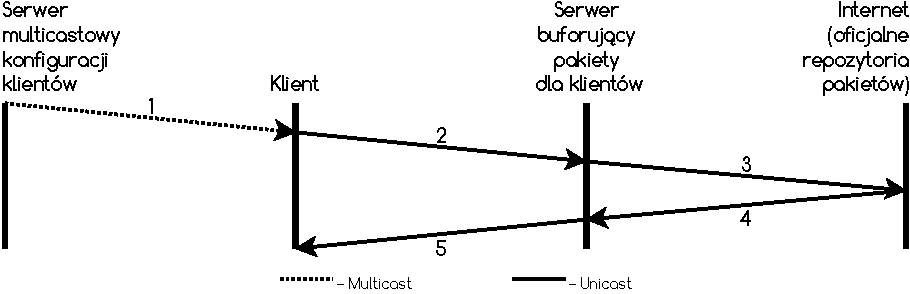
\includegraphics[width=\textwidth]{img/schemat-komunikacji}
%	\caption{Schemat komunikacji klienta i~serwera (lub~serwerów --- w~zależności od~konfiguracji)}
%	\label{fig:schemat-komunikacji}
%\end{figure}
%
%Jeśli w~chwili~$t$ serwer rozkazał swoim klientom instalację zbioru pakietów~$A$ i~klient~$X$ zainstalował te~pakiety przed chwilą~$t+1$, w~której serwer rozkazał instalację pewnego zbioru pakietów~$B$, to~jeśli:\mynobreakpar
%
%\begin{itemize}
%	\item $A=B$, to~w~chwili~$t+1$ klient niczego nie zmienia w~swojej konfiguracji\footnote{Chyba, że~serwer rozkazał również aktualizację zainstalowanego już oprogramowania klientów, ale~to wykluczamy na~potrzeby tych rozważań.}. Warto zauważyć, że~w praktyce sytuacja, w~której~$A=B$, zdarza się najczęściej, ponieważ typowe czasy rozgłaszania konfiguracji serwera to~kilkadziesiąt minut\footnote{Np.~w~\hyperref[sec:puppet]{Puppet} domyślny czas między synchronizacjami z~serwerem wynosi~30~minut.} lub~kilka godzin, podczas gdy~administrator sieci zazwyczaj nie zmienia tak często rozgłaszanej konfiguracji klientów.
%	\item $A\neq B\;\wedge\;\exists_{p\in A}\;p\not\in B$, to~klient niczego nie zmienia w~swojej konfiguracji, w~szczególności nie odinstalowuje pakietu~$p$ --- klient odinstalowuje tylko te~pakiety, które są~\emph{explicite} wymienione na~liście pakietów do~usunięcia.
%	\item $A\neq B\;\wedge\;\exists_{p\in B}\;p\not\in A$, to~klient instaluje pakiet~$p$.
%\end{itemize}
%
%Konfiguracja serwera pozwala opcjonalnie włączyć multicastowe rozgłaszanie listy wszystkich obsługiwanych multicastowych adresów~IP i~odpowiadających im~opisowych nazw, ustalonych przez administratora sieci, dzięki czemu aplikacja klienta jest zdolna wyświetlić wszystkie adresy multicastowe\footnote{Zakres multicastowych adresów~IP jest regulowany przez \gls{iana} w~\href{https://tools.ietf.org/html/rfc5771}{RFC5771} i~jest następujący: 224.0.0.0 -- 239.255.255.255~(\href{https://en.wikipedia.org/wiki/Classful_network\#Classful_addressing_definition}{klasa~D}), przy~czym adresy z~zakresu 224.0.0.0 -- 224.0.0.255 \href{https://www.iana.org/assignments/multicast-addresses/multicast-addresses.xhtml}{są}~wykorzystywane m.in.~przez protokoły trasowania oraz~protokoły wykrywające topologię sieci i~nie są~wykorzystywane przez aplikacje~\cite{rfc5771}.}, na~których rozgłaszane są~konfiguracje klientów. Przykładowo, dla~sieci przedstawionej na~rys.~\ref{fig:simple-network}, lista zwrócona przez serwer~(tu~zapisaną w~notacji znanej np.~z~języka Python) byłaby następująca:\mynobreakpar
%\begin{lstlisting}[language=Python,numbers=none,frame=none]
%[
%	[ { 'name' : 'Laboratorium A' }, { 'IP' : '224.10.10.1' } ],
%	[ { 'name' : 'Laboratorium B' }, { 'IP' : '224.10.10.2' } ],
%	[ { 'name' : 'Laboratorium C' }, { 'IP' : '224.10.10.3' } ],
%	[ { 'name' : 'Biblioteka'     }, { 'IP' : '224.10.10.4' } ]
%]
%\end{lstlisting}
%
%\begin{figure}
%	\centering
%	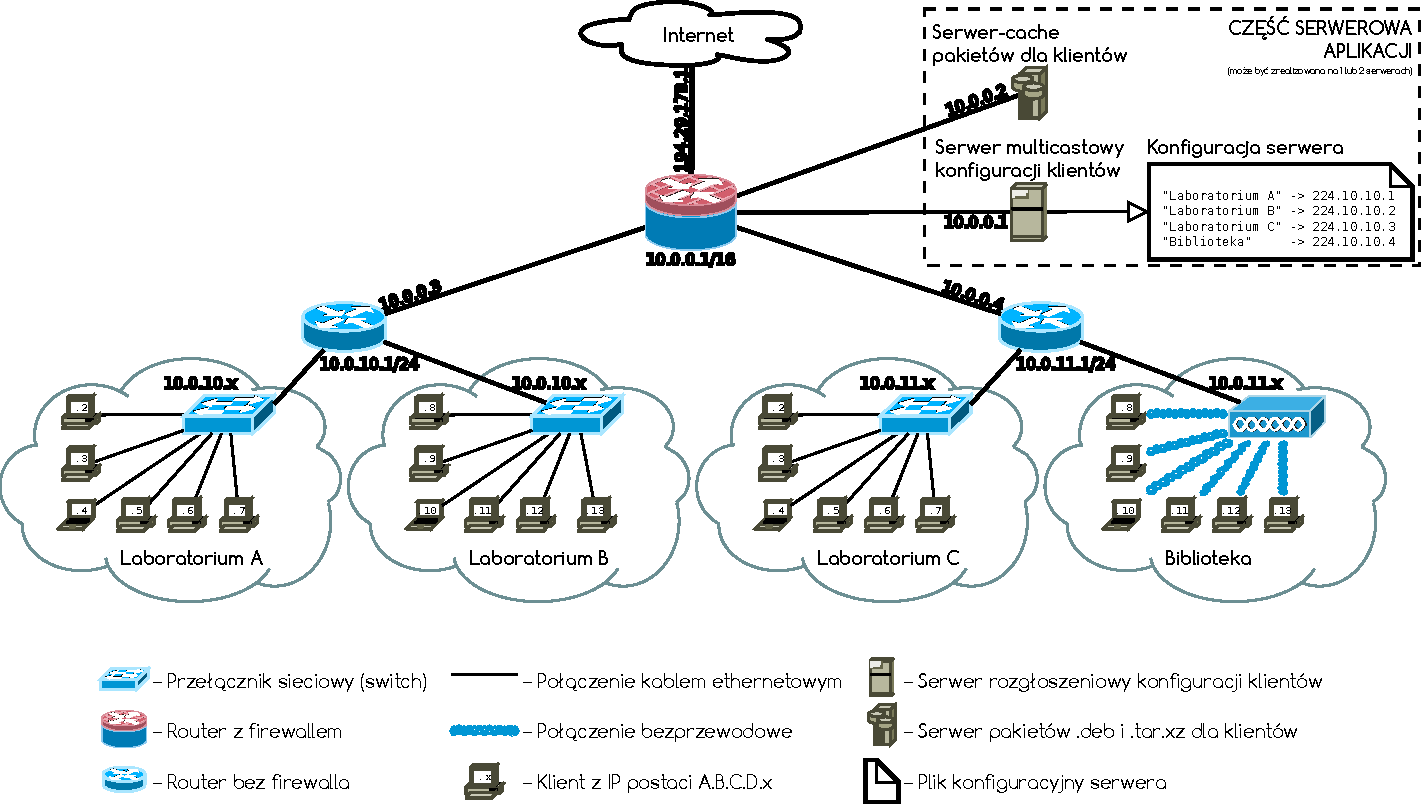
\includegraphics[width=\textwidth]{img/przykladowa-siec-wireless}
%	\caption{Przykładowa sieć działająca pod~kontrolą serwerów dystrybucji oprogramowania}
%	\label{fig:simple-network}
%\end{figure}

%------------------------------------------------------------------------------

\section{Wnioski}

TODO

\end{document}
